\section{Laufzeitsicht}
\subsection{Spielerdaten laden}
\begin{figure}
    \centering
    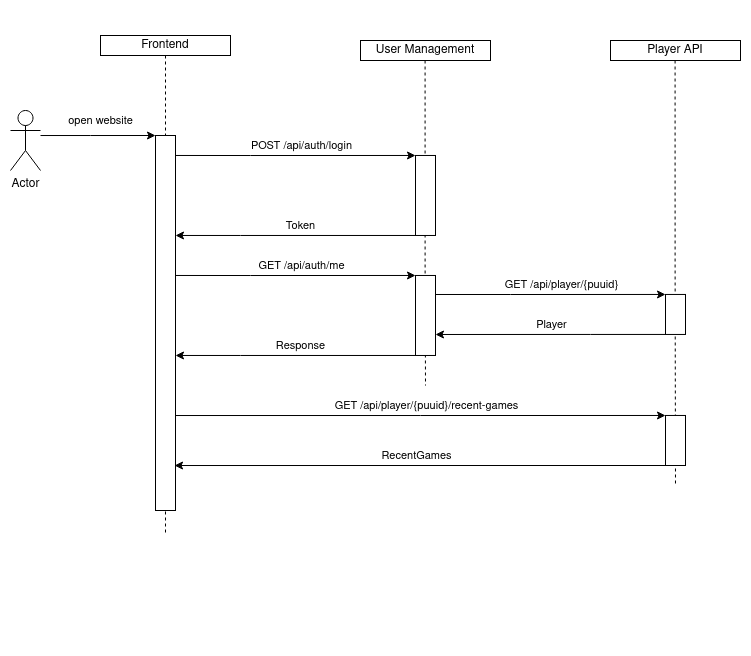
\includegraphics[width=\textwidth]{cdc-07-dynamic-get_own_data.drawio}
    \caption{Sequenzdiagramm für das Laden von Spielerdaten}
    \label{fig:load-data}
\end{figure}

In Abbildung~\ref{fig:load-data} ist der Ablauf gezeigt, welche Http Requests gesendet werden, wenn sich ein Spieler
der schon einen Account hat und dessen Spiele schon importiert sind, einloggt.


\subsection{Neuer Spieler importieren}

Um einen neuen Spieler zu importieren, wird eine Anfrage von dem Frontend an die Player-API gesendet.
Da diese Anfrage zustandslos ist, werden regelmäßig HTTP-Anfragen gesendet, um den aktuellen Import-Status
zu erhalten.
Diese Informationen werden im Frontend an den entsprechenden stellen dargestellt.
Im Player-API Service wird für den Import ein Backgroundtask gestartet, der über einen grpc Stream den Import im
Games Importer Service startet und die Anzahl der importierten Spiele streamt.

\graphic{cdc-07-import-player.drawio}{Flussdiagramm des Spieler imports}

\subsection{Spieler vergleichen}

Das Diagramm in Abbildung~\ref{fig:compare-diagram} stellt den Ablauf dar, wenn sich ein Spieler mit anderen Spielern vergleichen will.

\begin{figure}[H]
    \centering
    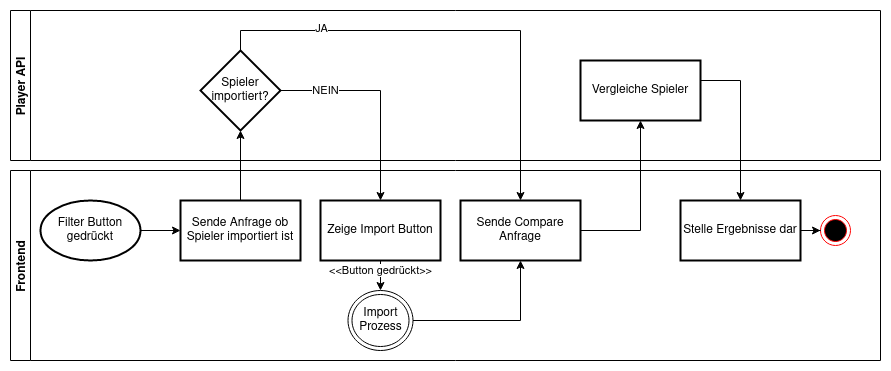
\includegraphics[width=\textwidth]{cdc-07-compare.drawio}
    \caption{Swimlane Diagramm zum Vergleich von Spielern}
    \label{fig:compare-diagram}
\end{figure}

\subsection{Error handling}
\subsubsection{Game importing}
Beim importieren des Spiels können wie in \ref{riot-api-libraries} bereits erklärt verschiedene Fehler auftreten. Damit Fehler, die von der Riot API kommen und meist nur temporär sind, nicht den Service zum Absturz bringen, werden alle API Aufrufe innerhalb einer try, except Anweisung ausgeführt. Sollte dann ein API Aufruf zu einem Fehler führen, so wird dieser bei Fehlern wie 503 - Service Unavailable wiederholt. Bei Fehlern, die nicht temporär sind (400 - Bad Request) wird der Request verworfen.\\
Auch die Datenbank kann Errors liefern, weshalb auch alle Datenbank Anfragen innerhalb von try, except Anweisung laufen. Tritt hierbei ein Fehler auf, so wird die komplette Anfrage die zu diesem geführt hat (zB das importieren eines Spiels) abgebrochen, so dass der Service weitere Anfragen verarbeiten kann. Wird ein Ablauf, wie das importieren eines Spiels unterbrochen, so wird dieser im nächsten update Durchlauf erneut versucht.

\subsubsection{Monitoring}

Um die Applikation zu monitoren, werden verschiedene Tools verwendet.

\textbf{sentry} (\href{https://sentry.io/}{https://sentry.io/}) wird verwendet, um Fehler zentral zu tracken und
Alerts zu verschicken.
Sentry wurde für alle Backend Services eingerichtet um einen Überblick über serverseitiges Fehlverhalten zu bekommen.

Um die Performance von Requests zu tracken, wird \textbf{SigNoz} (\href{https://signoz.io/}{https://signoz.io/}) verwendet.
Damit werden Traces für Anfragen erstellt, womit festgestellt werden kann wie lange Anfragen brauchen und welche Methode wie lange braucht.
Außerdem werden automatisch Datenbank Operationen gemessen, wodurch es möglich ist zwischen Applikationslogik
und Datenbank Operationen zu unterscheiden, wie in Abbildung~\ref{fig:signoz-traces} zu sehen ist.
\begin{figure}[H]
    \centering
    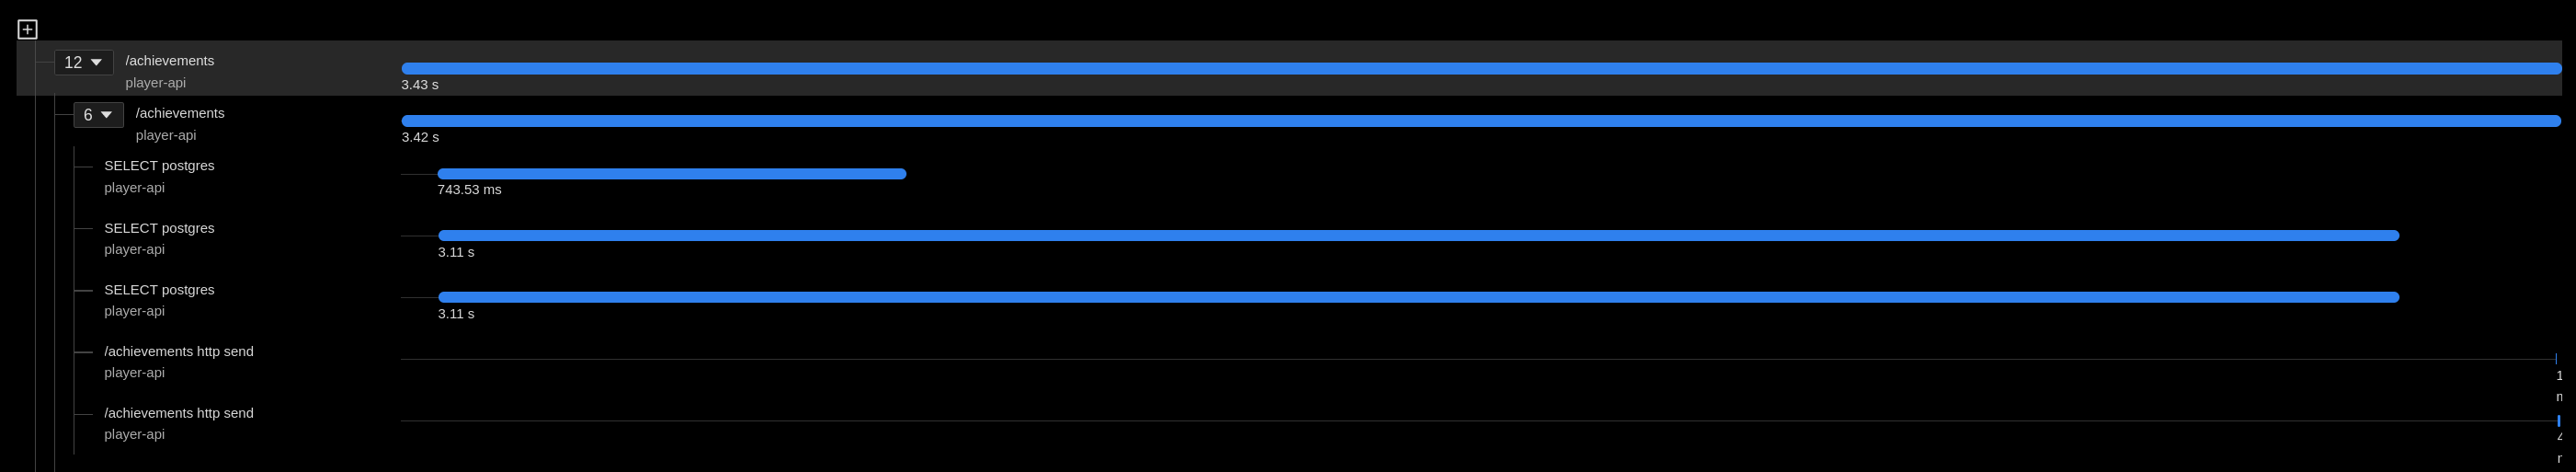
\includegraphics[width=\textwidth]{signoz_traces}
    \caption{Trace Details in SigNoz zu einem /achievements Request}
    \label{fig:signoz-traces}
\end{figure}